\documentclass[10pt,a4paper]{article}
\usepackage[utf8]{inputenc}
\usepackage{amsmath}
\usepackage{bm}
\usepackage{amsfonts}
\usepackage{amssymb}
\usepackage{tikz}
\usepackage[left=2cm,right=2cm,top=2cm,bottom=2cm]{geometry}
\usepackage{graphicx}
\usepackage{subcaption}

\usepackage{algorithm}
\usepackage[noend]{algpseudocode}
\makeatletter
\def\BState{\State\hskip-\ALG@thistlm}
\makeatother

\usepackage{listings}
\usepackage{color}

\definecolor{mygreen}{rgb}{0,0.6,0}
\definecolor{mygray}{rgb}{0.5,0.5,0.5}
\definecolor{mymauve}{rgb}{0.58,0,0.82}

\lstset{ 
  backgroundcolor=\color{white},   % choose the background color; you must add \usepackage{color} or \usepackage{xcolor}; should come as last argument
  basicstyle=\footnotesize,        % the size of the fonts that are used for the code
  breakatwhitespace=false,         % sets if automatic breaks should only happen at whitespace
  breaklines=true,                 % sets automatic line breaking
  captionpos=b,                    % sets the caption-position to bottom
  commentstyle=\color{mygreen},    % comment style
  deletekeywords={...},            % if you want to delete keywords from the given language
  escapeinside={\%*}{*)},          % if you want to add LaTeX within your code
  extendedchars=true,              % lets you use non-ASCII characters; for 8-bits encodings only, does not work with UTF-8
  frame=single,	                   % adds a frame around the code
  keepspaces=true,                 % keeps spaces in text, useful for keeping indentation of code (possibly needs columns=flexible)
  keywordstyle=\color{blue},       % keyword style
  language=Octave,                 % the language of the code
  morekeywords={*,...},            % if you want to add more keywords to the set
  numbers=left,                    % where to put the line-numbers; possible values are (none, left, right)
  numbersep=5pt,                   % how far the line-numbers are from the code
  numberstyle=\tiny\color{mygray}, % the style that is used for the line-numbers
  rulecolor=\color{black},         % if not set, the frame-color may be changed on line-breaks within not-black text (e.g. comments (green here))
  showspaces=false,                % show spaces everywhere adding particular underscores; it overrides 'showstringspaces'
  showstringspaces=false,          % underline spaces within strings only
  showtabs=false,                  % show tabs within strings adding particular underscores
  stepnumber=1,                    % the step between two line-numbers. If it's 1, each line will be numbered
  stringstyle=\color{mymauve},     % string literal style
  tabsize=2,	                   % sets default tabsize to 2 spaces
  title=\lstname                   % show the filename of files included with \lstinputlisting; also try caption instead of title
}

\newcommand{\drm}{\mathrm{d}}

\begin{document}

\title{Optimal Control of the Poisson Equation with OpenFOAM}
\author{Victor Hernández-Santamaría \thanks{University of Deusto} \and José Vicente Lorenzo Gómez \thanks{Universidad Autónoma de Madrid.}}

\maketitle

In this tutorial, we show how to use the C++ library OpenFOAM (Open Field Operation and Manipulation) in order to solve control problems for partial differential equations (PDE). 

OpenFOAM is a free open source toolbox that allows the user to code customized solvers for Continuum Mechanics, with special attention to the field of Computational Fluid Dynamics. One can either use one of the multiple solvers already programmed for steady-state, transient or multiphase problems in fluid mechanics, or code his own solver depending on particular needs.

In this work, we will solve the optimal control problem
%
\begin{equation} \label{eq:CostFunctional}
\min _{u \in L^2 \left( \Omega \right)} \mathcal{J}\left( u\right) = \min _{u \in L^2 \left( \Omega \right)} \frac{1}{2} \int_{\Omega} \left( y - y_d \right) ^2 \drm \Omega + \frac{\beta}{2} \int_{\Omega} u ^2 \drm \Omega,
\end{equation}
%
where $u$ is the control variable, $y$ the state variable and $y_d$ a target function. The minimization problem is subject to the elliptic partial differential equation
%
\begin{equation} \label{eq:PoissonEq}
\begin{cases}
-\Delta y  = f + u & \text{in } \Omega, \\
y = 0 & \text{on } \Gamma.
\end{cases}
\end{equation}

We use some classical gradient descent methods based on the adjoint methodology, namely the steepest descent and conjugate gradient methods. The corresponding adjoint system for \eqref{eq:PoissonEq} writes as,
%
\begin{equation} \label{eq:PoissonAdjointEq}
\begin{cases}
- \Delta \lambda = y - y_d & \text{in } \Omega,  \\
\lambda = 0 & \text{on } \Gamma.
\end{cases}
\end{equation}

In the steepest descent gradient method, we compute the directional derivative of the cost function in \eqref{eq:CostFunctional},
%
\begin{equation}
\mathcal{D}_{ \delta u} \mathcal{J} \left( u \right) = \int_{\Omega} \left( \lambda + \beta u \right) \delta u \drm \Omega,
\end{equation}
%
where $\lambda$ is solution to the elliptic problem in \eqref{eq:PoissonAdjointEq}, and use the gradient to update the control variable as
%
\begin{equation}
u^{\left( n + 1 \right)} = u^{\left( n \right)} - \gamma \left( \lambda^{\left( n \right)} + \beta u^{\left( n \right)} \right),
\end{equation}
%
for some value of $\gamma$.

One of the main advantages of OpenFOAM is its friendly syntax to describe PDE, as can be seen in the lines 10 and 13 in the code below.

\lstinputlisting[language=C++]{steepestdescent.cpp}

In order to improve the covergence to the optimal control, the conjugate gradient method is applied also to the problem. First, the state variable must be separated in two terms as
%
\begin{equation}
y = y_u + y_{f},
\end{equation}
%
where $y_u$ solves the state equation with zero Dirichlet boundary conditions,
%
\begin{equation} \label{eq:PoissonEqu}
\begin{cases}
-\Delta y_u  = u & \text{in } \Omega, \\
y_u = 0 & \text{on } \Gamma,
\end{cases}
\end{equation}
%
and $y_{f}$ is the control-free solution to the state equation,
%
\begin{equation} \label{eq:PoissonEq0}
\begin{cases}
-\Delta y_{f}  = f & \text{in } \Omega, \\
y_{f} = 0 & \text{on } \Gamma.
\end{cases}
\end{equation}

Now, using the above separation of the state variable, one part depending on the control and the other part on a known source term, the cost functional in \eqref{eq:CostFunctional} can be expressed as
%
\begin{equation} \label{eq:CostFunctionalcg}
\mathcal{J} \left( u \right) = \frac{1}{2} \left( y_u + y_f - y_d, y_u + y_f - y_d \right)_{L^2\left( \Omega \right)} + \frac{\beta}{2} \left( u , u \right) _{L^2\left( \Omega \right)}.
\end{equation}

We define a linear operator $\Lambda: L^2\left( \Omega \right) \rightarrow L^2\left( \Omega \right)$ that takes a control $u$ and returns the solution to problem \eqref{eq:PoissonEqu}-\eqref{eq:PoissonBCu}, so that $y_u = \Lambda u$. We introduce as well its adjoint operator $\Lambda^*: L^2\left( \Omega \right) \rightarrow L^2\left( \Omega \right)$ that takes the source term in \eqref{eq:PoissonAdjointEq} and solves the Poisson equation, so that $\lambda = \Lambda^* \left( y - y_d \right)$.

The directional derivative of the functional \eqref{eq:CostFunctionalcg} then reads as
%
\begin{equation}
\mathcal{D}_{\delta u} \mathcal{J}\left( u \right) = \left( \underbrace{ \left(  \Lambda^* \Lambda + \beta I  \right)}_{A_{cg}} u - \underbrace{ \Lambda^* \left( y_d - y_f \right)}_{b_{cg}}, \delta u \right) _{L^2\left( \Omega \right)}.
\end{equation}

After having identified $A_{cg}$ and $b_{cg}$ we can use the conjugate gradient method to reach the optimal control faster. 

\begin{algorithm}[h]
\caption{Optimal control with Conjugate Gradient Method}\label{CGalgorithm}
\begin{algorithmic}[1]
\Require $y_D$, $u^{\left(0\right)}$, $\beta$, $y_d$, $tol$
\State $n \gets 0 $
\State compute the control-free solution, $y_f$
\State $b \gets \Lambda^*\left( y_d - y_f \right)$
\State $z \gets \Lambda u$
\State $g \gets \Lambda^*z + \beta u - b$
\State $h \gets ||g||^2_{L^2\left(\left[0,T\right]\right)}$
\State $h_a \gets h$
\State $r \gets -g$
\While{$||r||_{L^2\left(\left[0,T\right]\right)} > tol $}
\State $z \gets \Lambda r$
\State $w \gets \Lambda^*z + \beta r$
\State $\alpha \gets \frac{h}{\left(r,w\right)_{L^2\left(\left[0,T\right]\right)}}$
\State $u \gets u + \alpha r$
\State $g \gets g + \alpha w$
\State $h_a \gets h$
\State $h \gets ||g||^2_{L^2\left(\left[0,T\right]\right)}$
\State $\gamma \gets \frac{h}{h_a}$
\State $r \gets -g + \gamma r$
\State $n \gets n + 1$
\EndWhile

\end{algorithmic}
\end{algorithm}

\lstinputlisting[language=C++]{conjugategradient.cpp}

Both solvers, \textit{laplaceAdjointFoam} for the steepest descent method with $\gamma = 10$ and \textit{laplaceCGAdjointFoam} for the conjugate gradient method, have been tested in a square domain $[0, 1] \times [0, 1]$ with zero Dirichlet boundary conditions and $\beta = 10^{-3},10^{-4},10^{-5},10^{-6}$. The target function is $y_d = xy \sin \left( \pi x \right) \sin \left( \pi y \right)$. 

The problem setup is called \textit{case} in OpenFOAM and it is independent from the solver itself. A typical case in OpenFOAM has three folders: \textit{0}, where the problem fields are stored along with their boundary conditions; \textit{constant}, that includes the mesh data and the physical properties; and \textit{system}, with parameters regarding the numerical solution and problem ouput such as tolerances, linear solvers or write interval. In this example, the case folder is called \textit{laplaceAdjointFoamCase}.

\begin{figure}[h]
    \centering
    \begin{subfigure}[b]{0.4\textwidth}
        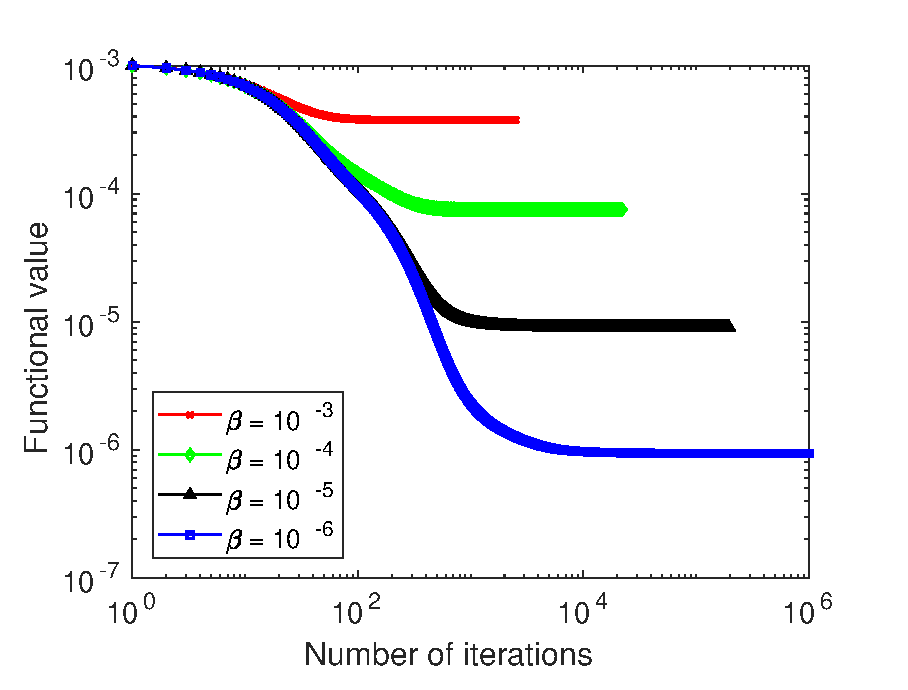
\includegraphics[width=\textwidth]{sd_J.eps}
        \caption{Steepest descent method.}
        \label{fig:SDcostviterations}
    \end{subfigure}
    ~ %add desired spacing between images, e. g. ~, \quad, \qquad, \hfill etc. 
      %(or a blank line to force the subfigure onto a new line)
    \begin{subfigure}[b]{0.4\textwidth}
        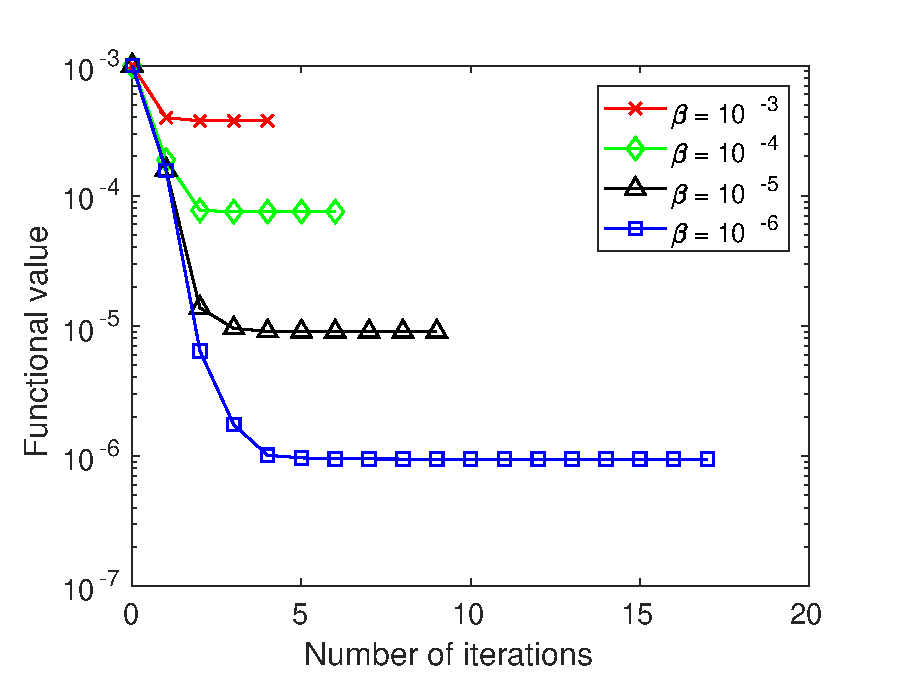
\includegraphics[width=\textwidth]{cg_J.eps}
        \caption{Conjugate gradient method.}
        \label{fig:CGcostviterations}
    \end{subfigure}
    ~ %add desired spacing between images, e. g. ~, \quad, \qquad, \hfill etc. 
    %(or a blank line to force the subfigure onto a new line)
    \caption{Functional value against the number of iterations of the gradient method.}\label{fig:Results1}
\end{figure}

\begin{figure}[h]
    \centering
    \begin{subfigure}[b]{0.4\textwidth}
        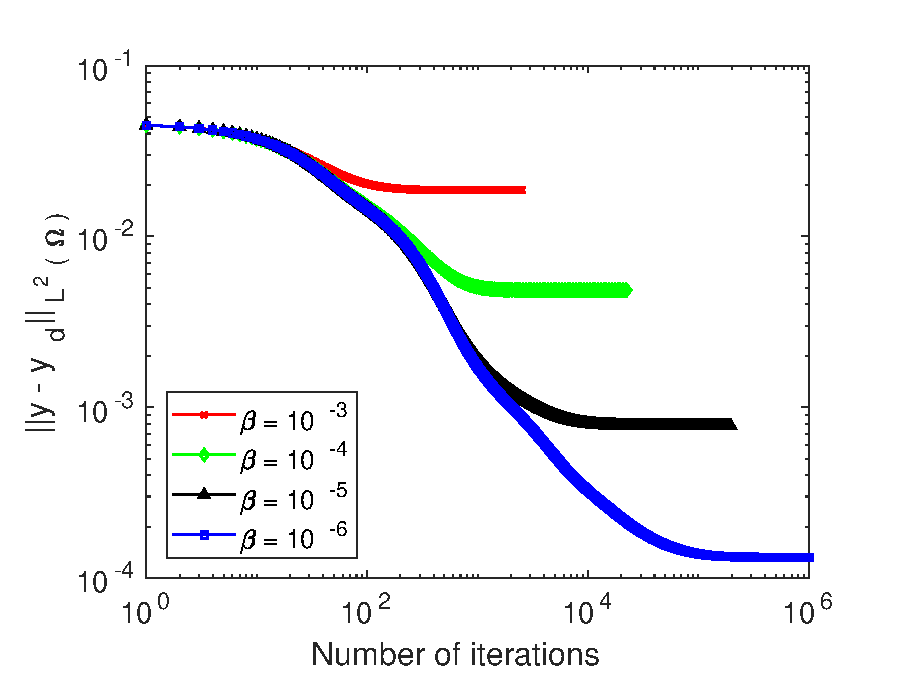
\includegraphics[width=\textwidth]{sd_Jy.eps}
        \caption{Steepest descent method.}
        \label{fig:SDcostviterations}
    \end{subfigure}
    ~ %add desired spacing between images, e. g. ~, \quad, \qquad, \hfill etc. 
      %(or a blank line to force the subfigure onto a new line)
    \begin{subfigure}[b]{0.4\textwidth}
        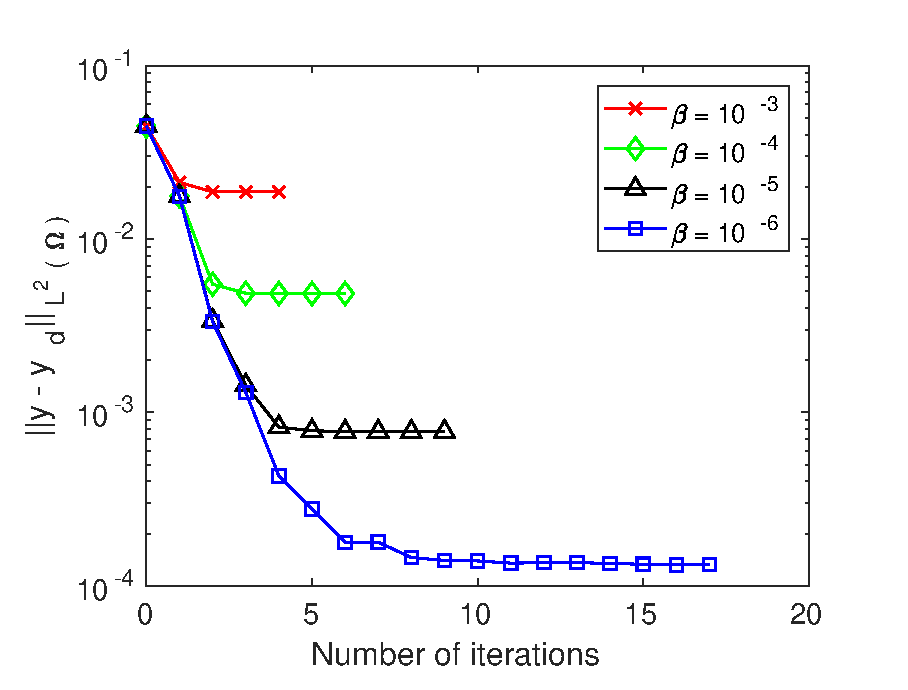
\includegraphics[width=\textwidth]{cg_Jy.eps}
        \caption{Conjugate gradient method.}
        \label{fig:CGcostviterations}
    \end{subfigure}
    ~ %add desired spacing between images, e. g. ~, \quad, \qquad, \hfill etc. 
    %(or a blank line to force the subfigure onto a new line)
    \caption{$|| y - y_d ||_{L^2 \left( \Omega \right)}$ against the number of iterations of the gradient method.}\label{fig:Results1}
\end{figure}

\begin{thebibliography}{1}
\bibitem{openfoam}
\textit{The OpenFOAM Foundation}, openfoam.org.
\bibitem{troltzsch}
F. Tröltzsch. \textit{Optimal control of partial differential equations: theory, methods, and applications}. American Mathematical Soc., 2010.
\end{thebibliography}

\end{document}